%%%%%%%%%%%%%%%%%%%%%%%%%%%%%%%%%%%%%%%%%
% Beamer Presentation
% LaTeX Template
% Version 1.0 (10/11/12)
%
% This template has been downloaded from:
% http://www.LaTeXTemplates.com
%
% License:
% CC BY-NC-SA 3.0 (http://creativecommons.org/licenses/by-nc-sa/3.0/)
%
%%%%%%%%%%%%%%%%%%%%%%%%%%%%%%%%%%%%%%%%%

%----------------------------------------------------------------------------------------
%	PACKAGES AND THEMES
%----------------------------------------------------------------------------------------

\documentclass{beamer}

\mode<presentation> {

% The Beamer class comes with a number of default slide themes
% which change the colors and layouts of slides. Below this is a list
% of all the themes, uncomment each in turn to see what they look like.

%\usetheme{default}
% \usetheme{AnnArbor}
% \usetheme{Antibes} +
% \usetheme{Bergen}
% \usetheme{Berkeley}
% \usetheme{Berlin}
% \usetheme{Boadilla}
% \usetheme{CambridgeUS}
% \usetheme{Copenhagen} +
% \usetheme{Darmstadt}
% \usetheme{Dresden}
% \usetheme{Frankfurt}
% \usetheme{Goettingen}
% \usetheme{Hannover}
% \usetheme{Ilmenau}
% \usetheme{JuanLesPins}
% \usetheme{Luebeck} +
% \usetheme{Madrid}
\usetheme{Malmoe}
% \usetheme{Marburg}
% \usetheme{Montpellier} +
% \usetheme{PaloAlto}
% \usetheme{Pittsburgh}
% \usetheme{Rochester}
% \usetheme{Singapore}
% \usetheme{Szeged}
% \usetheme{Warsaw} +

% As well as themes, the Beamer class has a number of color themes
% for any slide theme. Uncomment each of these in turn to see how it
% changes the colors of your current slide theme.

% \usecolortheme{albatross}
% \usecolortheme{beaver}
% \usecolortheme{beetle}
% \usecolortheme{crane}
% \usecolortheme{dolphin}
% \usecolortheme{dove}
% \usecolortheme{fly}
% \usecolortheme{lily}
% \usecolortheme{orchid}
% \usecolortheme{rose}
% \usecolortheme{seagull}
% \usecolortheme{seahorse}
\usecolortheme{whale}
% \usecolortheme{wolverine}

%\setbeamertemplate{footline} % To remove the footer line in all slides uncomment this line
%\setbeamertemplate{footline}[page number] % To replace the footer line in all slides with a simple slide count uncomment this line

%\setbeamertemplate{navigation symbols}{} % To remove the navigation symbols from the bottom of all slides uncomment this line
}

\usepackage{graphicx} % Allows including images
\usepackage{booktabs} % Allows the use of \toprule, \midrule and \bottomrule in tables
\usepackage[brazil]{babel}
\selectlanguage{brazil}
\languagepath{brazil}
\deftranslation[to=brazil]{Example}{Exemplo}
\deftranslation[to=brazil]{Theorem}{Teorema}
\usepackage[utf8]{inputenc}
\usepackage{amssymb}
\usepackage{mathtools}
\usepackage{pythonhighlight}

%----------------------------------------------------------------------------------------
%	TITLE PAGE
%----------------------------------------------------------------------------------------

\title[Identificação de Locutor]{Identificação de Locutor} % The short title appears at the bottom of every slide, the full title is only on the title page

\author{Ramon Duarte de Melo \& André Ribeiro Queiroz} % Your name
\institute[UFRJ] % Your institution as it will appear on the bottom of every slide, may be shorthand to save space
{
    Universidade Federal do Rio de Janeiro \\ % Your institution for the title page
    \medskip
    \textit{ramonduarte@poli.ufrj.br \& handre\_queiroz@poli.ufrj.br} % Your email address
}
\date{\today} % Date, can be changed to a custom date

\begin{document}

\begin{frame} % SLIDE 1
    \titlepage % Print the title page as the first slide
\end{frame}

\begin{frame} % SLIDE 2
    \frametitle{Sumário} % Table of contents slide, comment this block out to remove it
    \tableofcontents 
\end{frame}

%----------------------------------------------------------------------------------------
%	PRESENTATION SLIDES
%----------------------------------------------------------------------------------------

%------------------------------------------------
\section{O Problema} 
%------------------------------------------------

\begin{frame} % SLIDE 3
    \frametitle{Objetivo}
    
    Usar biometria de voz para identificar quem está falando

    \begin{figure}[]
        \centering
        
\includegraphics[width=\linewidth]{fig1.jpg}
    \end{figure}
\end{frame}

\begin{frame} % SLIDE 3
    \frametitle{O Sinal de Voz}
    
    O sinal de áudio recebido como entrada é produzido através de diversas transformações que ocorrem em estágios distintos da captação sonora.
    Portanto, precisamos extrair somente as propriedades sonoras chamadas de "dependentes do locutor".

    \medskip

    Este processamento é geralmente feito por técnicas de parametrização, como o LPC (\emph{Linear Prediction Coding}):

    \bigskip

    \begin{math}
        s(n) = - \sum_{k=1}^{p} a_{k} \cdot s(n-k) + e(n)
    \end{math}

    \bigskip

    \begin{itemize}
        \item $p$ é a ordem de predição;

        \item $a_{k}$  são os coeficientes de predição
    
        \item $s(n-k)$ são ps sinais anteriores
    
        \item $e(n)$ é o erro de predição.
    \end{itemize}

    


\end{frame}

\section{Pipeline}

\subsection{Diagrama}

\begin{frame} % SLIDE 3
    \frametitle{Visão Geral do Sistema}

    \begin{figure}
        \centering
        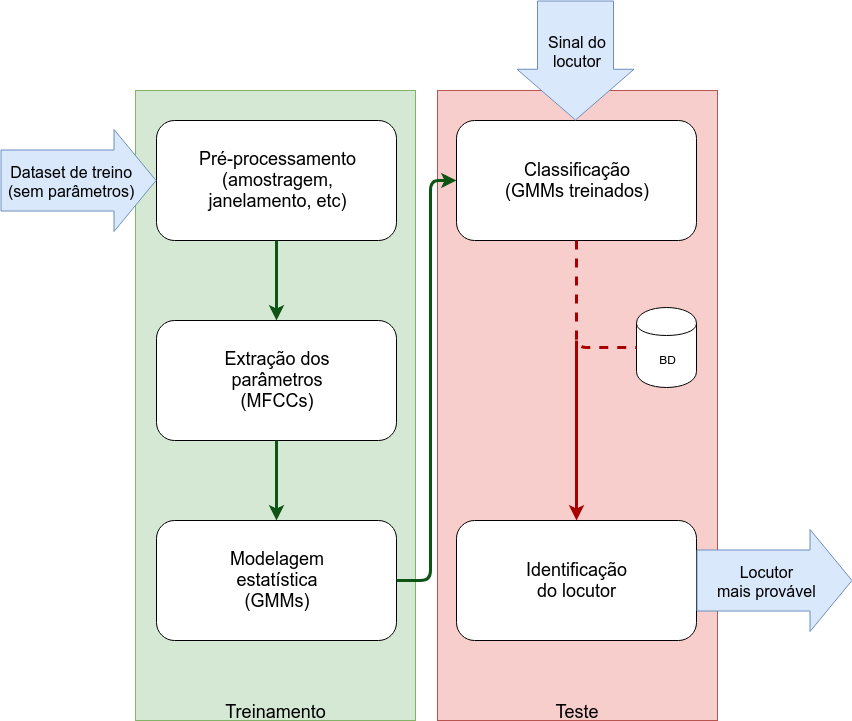
\includegraphics[height=192pt]{fig2.png}
        % \caption{Pipeline do processo de reconhecimento de locutor.}
    \end{figure}


\end{frame}


\subsection{Dados de entrada}

\begin{frame} % SLIDE 3
    \frametitle{Captação do sinal}

    \begin{itemize}
        \item Áudios de entrada amostrados em 8kHz ou 16kHz 
        \medskip
        \item 16 bits por amostra
        \medskip
        \item Duração variável entre 10 e 60 segundos
    \end{itemize}

    
\end{frame}

\begin{frame} % SLIDE 3
    \frametitle{\emph{Datasets}}

    Dataset de treinamento: 34 locutores, 5 frases para cada locutor, 20-30 segundos

    Dataset de teste: os mesmos 34 locutores, 1 frase para cada, $\approx$10 segundos

\end{frame}

\subsection{Pré-processamento}

\begin{frame} % SLIDE 3
    \frametitle{Amostragem}

    O sinal de voz é tradicionalmente não-estacionário, o que dificulta a análise das frequências contidas nele. 

    \begin{figure}[]
        \centering
        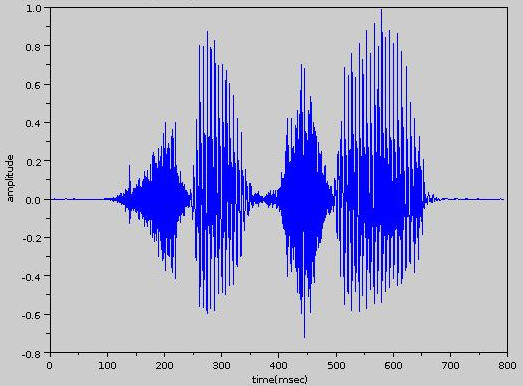
\includegraphics[height=135pt]{fig4.png}
        \centering

    \end{figure}
\end{frame}


\begin{frame} % SLIDE 3
    \frametitle{Amostragem}

    O sinal de áudio é dividido em quadros de 20-30 ms para encontrar estacionariedade.

    \begin{figure}[]
        \centering
        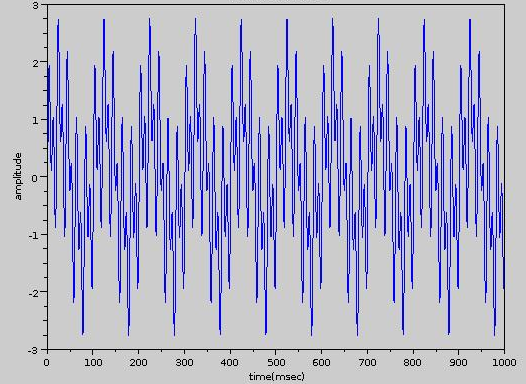
\includegraphics[height=135pt]{fig3.png}
        \centering

    \end{figure}

\end{frame}

\begin{frame} % SLIDE 3
    \frametitle{Janelamento}

    Como o intervalo de amostragem é arbitrário, o sinal apresenta descontinuidades nas extremidades da onda extraída.

    \begin{figure}[]
        \centering
        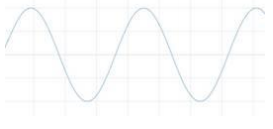
\includegraphics[height=135pt]{fig5.png}
        \centering

    \end{figure}
\end{frame}

\begin{frame} % SLIDE 3
    \frametitle{Janelamento}

    Para isso, é feito um janelamento que reduz as extremidades gradativamente a zero. 

    \begin{figure}[]
        \centering
        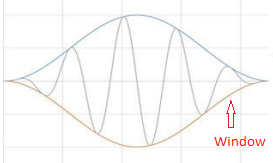
\includegraphics[height=135pt]{fig6.png}
        \centering

    \end{figure}
\end{frame}

\subsection{Treinamento}

\begin{frame} % SLIDE 3
    \frametitle{Parametrização}

    A extração dos parâmetros é feita pela técnica MFC (\emph{Mel-frequency cepstrum}):

    % diagrama: MFCCs are commonly derived as follows:[2]
    \begin{enumerate}
        \item Janelamento do sinal
        \item Transformada de Fourier das janelas
        \item Mapeamento das potências do espectro na escala de Mel
        \item Logaritmos das potências nas frequências de Mel
        \item Transformada discreta de cosseno dos logaritmos
        \item Obtenção das amplitudes do espectro resultante (são os MFCCs)
    \end{enumerate}

\end{frame}

\begin{frame} % SLIDE 3
    \frametitle{Modelagem}

    Pelo MFC, são extraídos 40 coeficientes (chamados de MFCCs), que alimentam GMMs (\emph{modelos misturados de gaussianas}).

    \medskip

    20 destes coeficientes são estáticos (constantes) e 20 são dinâmicos (diferenciais entre os coeficientes estáticos.)

    \medskip

    Durante o treinamento, os GMMs tentam aprender a distribuição dos MFCCs do dataset de treino.

    \medskip


    Durante o teste, os GMMs darão "notas" aos MFCCs do dataset de teste. 

\end{frame}

\begin{frame}[fragile] % SLIDE 3
    \frametitle{Modelagem}

    GMMs são modelos que agrupam linearmente $k$ distribuições normais para tentarem imitar a distribuição probabilística das subpopulações. Por isso, a identificação dos locutores consiste no locutor mais provável.

    \medskip

    Essa probabilidade $P(X|\lambda)$ é dada por:

    \bigskip

    \begin{math}
        P(X|\lambda) = \sum_{k=1}^{K} \omega_{k} P_{k}(X|\mu_{k}, \sum_{k})
    \end{math}

    \bigskip

    onde $P_{k}(X|\mu_{k}, \sum_{k})$ é a distribuição normal:

    \bigskip

    \begin{math}
        P_{k}(X|\mu_{k}, \sum_{k}) = (\sqrt{2\pi|\sum_{k}|})^{-1}e^{1/2(X-\mu_{k})^{T}\sum^{-1}(X-\mu_{k})}
    \end{math}

\end{frame}


\section{Implementação}

\subsection{MFC}

\begin{frame}[fragile] % SLIDE 3
    \frametitle{Módulos}

    Existem várias ferramentas que calculam MFCCs. Optamos pelo \texttt{python\_speech\_features}:

    \bigskip
    \begin{python}
import python_speech_features as mfc
from sklearn import preprocessing
def mfcc(sinal, taxa=16000, janela=0.03, dist_janelas=0.01):
    parametros = mfc.mfc(sinal, taxa, janela, dist_janelas)
    parametros = preprocessing.scale(parametros)
    return parametros
    \end{python}

\end{frame}

\subsection{GMM}

\begin{frame}[fragile] % SLIDE 3
    \frametitle{Módulos}

    Dos \texttt{parametros} extraídos anteriormente, apreendemos GMMs usando o módulo \texttt{sklearn}:

    \bigskip
    \begin{python}
from sklearn.mixture import GMM
gmm = GMM(n_components = 8, n_iter = 200, covariance_type='diag', n_init = 3)
gmm.fit(parametros)
    \end{python}

\end{frame}

\begin{frame}[fragile] % SLIDE 3
    \frametitle{Módulos}

    Em tese, o número de componentes e o total de iterações não deveriam ser arbitrários, mas sim descoberto através do algoritmo k-médias. 

    Para este trabalho, no entanto, optamos por utilizar os valores padrão:

    \begin{itemize}
        \item $k = 8$: os dados sempre terão 8 agrupamentos (e 8 centroides).
        \item 200 iterações: maioria dos exemplos utilizavam este valor.
    \end{itemize}

\end{frame}

\section{Conclusão}

\subsection{Planejamento Futuro}

\begin{frame}
    \frametitle{Objetos a serem testados}

    \begin{itemize}
        \item Datasets
        \item Parametrizações
        \item Modelagens estatísticas
        \item Ferramentas
        \item Pipelines
    \end{itemize}

\end{frame}


% \section{Referências bibliográficas}

% \begin{frame} % SLIDE 53
%     \frametitle{Referências bibliográficas}
%     \footnotesize{
%     \begin{thebibliography}{99} % Beamer does not support BibTeX so references must be inserted manually as below
%     % \bibitem[Smith, 2012]{p1} John Smith (2012)
%         \bibitem[Silberschatz, 2010]{p1}
%         Silberschatz, A., Korth, H. F., \& Sudarshan, S. (2010). Database system concepts (Vol. 4). New York: McGraw-Hill.

%         \bibitem[Rawat, 2017]{p2}
%         Rawat, U. (2017). Implementation of Locking in DBMS. Acessado a \date{25/11/2018} em https://www.geeksforgeeks.org/implementation-of-locking-in-dbms/.

%         \bibitem[Porfirio, 2013]{p3}
%         Porfirio, Alice \& Pellegrini, Alessandro \& Di Sanzo, Pierangelo \& Quaglia, Francesco. (2013). Transparent Support for Partial Rollback in Software Transactional Memories. 8097. 583-594. 10.1007/978-3-642-40047-6\_59. 

%         \bibitem[Poddar, 2013]{p4}
%         Poddar, Saumendra. (2003). SQL Server Transactions and Error Handling. Acessado a \date{25/11/2018} em https://www.codeproject.com/Articles/4451/SQL-Server-Transactions-and-Error-Handling.
%     \end{thebibliography}
%     }
% \end{frame}


% \begin{frame} % SLIDE 53
%     \frametitle{Referências bibliográficas}
%     \footnotesize{
%     \begin{thebibliography}{99} % Beamer does not support BibTeX so references must be inserted manually as below

%     \bibitem[Singhal, 2018]{p5}
%         Singhal, Akshay. (2018). Cascading Schedule | Cascading Rollback | Cascadeless Schedule. Acessado a \date{25/11/2018} em https://www.gatevidyalay.com/cascading-schedule-cascading-rollback-cascadeless-schedule/.

%         \bibitem[Pandey, 2018]{p6}
%         Pandey, Anand. (2018). Transactions and Concurrency Control. Acessado a \date{25/11/2018} em https://gradeup.co/transactions-and-concurrency-control-i-4c5d9b27-c5a7-11e5-bcc4-bc86a005f7ba.

% 	    \bibitem[Difference between, 2018]{p7}
%         Difference between. (2018). Difference between Deadlock and Starvation. Acessado a \date{25/11/2018} em http://www.differencebetween.info/difference-between-deadlock-and-starvation.

%     \end{thebibliography}
%     }
% \end{frame}

%------------------------------------------------

\end{document} 